% !TeX spellcheck = cs_CZ
\begin{example}\label{TEO:ex_10_8} Najděte odezvu napětí na kondenzátoru $u_c(t)$ obvodu na
  obrázku \ref{TEO:fig_cir_10_8} pro $t>0$. (zdroj \cite[s.~456]{Dorf}) 
  
  {\centering
   \captionsetup{type=figure}
   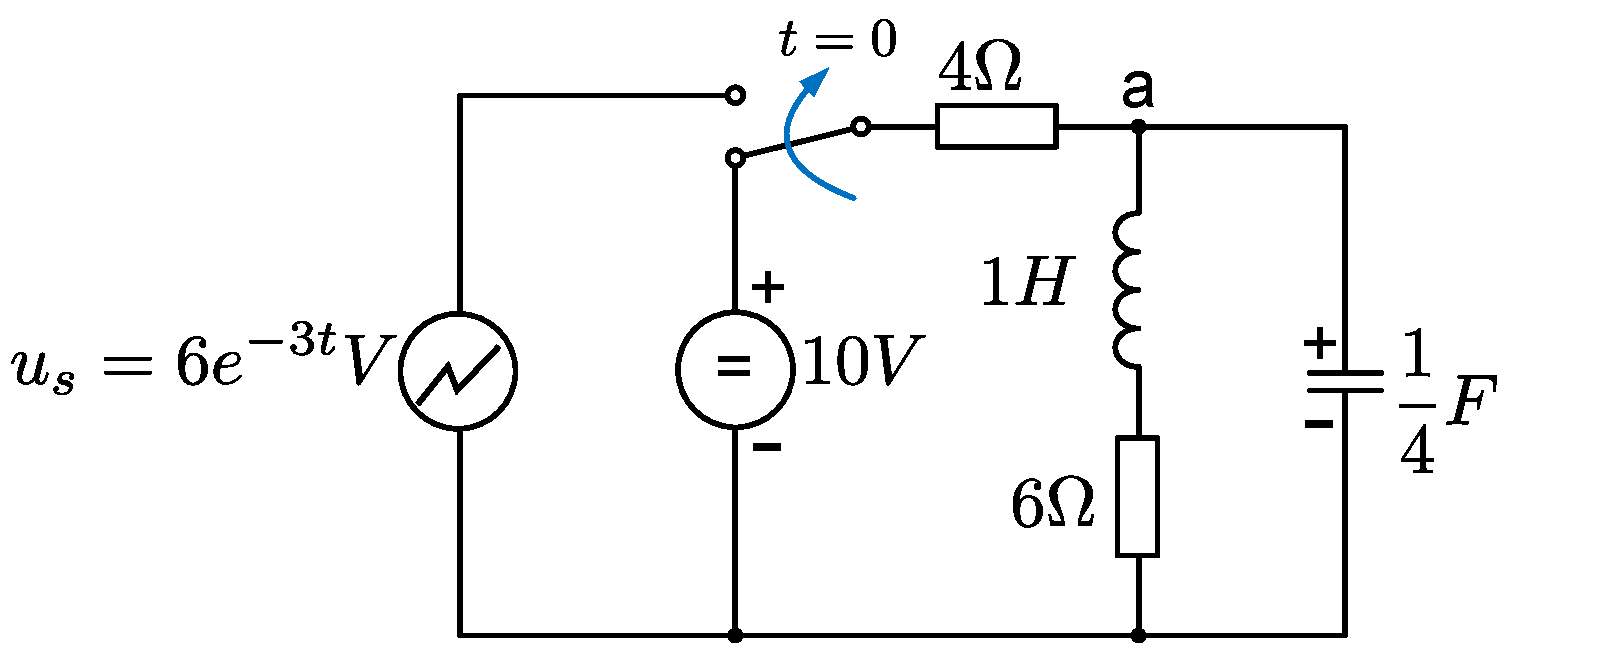
\includegraphics[width=1\linewidth]{response_ex10_8_RLC_cir.pdf}
   \captionof{figure}{Obvod k příkladu \ref{TEO:ex_10_8}}
   \label{TEO:fig_cir_10_8}
   \par}
  
  \textbf{Řešení:} Nejdříve stanovíme počáteční podmínky, které vyplývají z ustáleného stavu
  v době $t = 0^-$. Obvod na obr. \ref{TEO:fig_cir_10_8} můžeme překreslit do podoby na obr.
  \ref{TEO:fig_cir_10_8_steady} 
  
  {\centering
   \captionsetup{type=figure}
   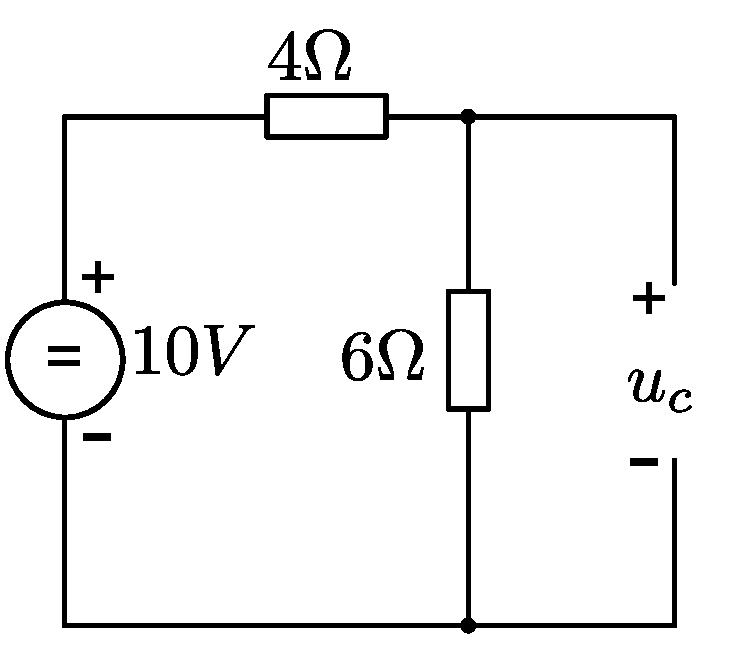
\includegraphics[width=0.4\linewidth]{response_ex10_8_steady.pdf}
   \captionof{figure}{Obvod k příkladu \ref{TEO:ex_10_8}}
   \label{TEO:fig_cir_10_8_steady}
   \par}
  \begin{equation}\label{TEO:eq_10_8_vysledek}
  u_c(t) = \frac{44}{3}e^{-2t}+\frac{1}{3}e^{-5t} - 9e^{-3t} \qquad [V]
  \end{equation}
\end{example}